\documentclass[11pt,a4paper]{article}
\usepackage[utf8]{inputenc}
\usepackage[utf8]{vietnam}
\usepackage{amsmath}
\usepackage{amsfonts}
\usepackage{amssymb}
\usepackage{xfrac}
\usepackage{indentfirst}
\usepackage{graphicx}
\usepackage{subfig}
\usepackage{enumerate}
\usepackage[left=1.5cm,right=1.5cm,top=1.5cm,bottom=1.5cm]{geometry}
\graphicspath{{images/}}
\usepackage[subpreambles=true]{standalone}
\usepackage{import}

\everymath{\displaystyle}

\title{\textbf{Bài tập Điều khiển quá trình \bigskip \\ Chủ đề Mô hình hóa lý thuyết}}
\author{Sưu tầm: Thi Minh Nhựt \and Email: thiminhnhut@gmail.com}
\date{Thời gian: \today}

\begin{document}

\maketitle

\section{Bài tập \ref{sec:baitap1-1binhchua}} \label{sec:baitap1-1binhchua}
    \paragraph{Giả thiết}
    Cho hệ thống như hình \ref{baitap1-1binhchua}: Biết lưu lượng ra $F_2$ tỉ lệ với chiều cao chất lỏng theo công thức $F_2 = R.h^{\sfrac{3}{2}}$ với $R$ là hằng số. Tiết diện của bồn chứa là $A$.
    \begin{figure}[htp]
        \begin{center}
            \subimport{images/}{baitap1-1binhchua.tex}
        \end{center}
        \caption{Hệ thống 1 bình chứa} \label{baitap1-1binhchua}
    \end{figure}

\paragraph{Yêu cầu}
    \begin{enumerate}[a.]
        \item Xác định các biến vào, biến ra, biến điều khiển, biến cần điều khiển và biến nhiễu.
        \item Viết phương trình động học cho mức chất lỏng trong bồn chứa.
        \item Tuyến tính hóa phương trình xây dựng được xung quanh vị trí cân bằng dựa trên phương pháp khai triển Taylor.
        \item Xác định hàm truyền $G(s) = \dfrac{H(s)}{F_1(s)}$
    \end{enumerate}

\paragraph{Bài giải}
    \begin{enumerate}[\it a.]
        \item \textit{Xác định các biến vào, biến ra, biến điều khiển, biến cần điều khiển và biến nhiễu.}
            \begin{itemize}
                \item Biến vào: $F_1, F_2$.
                \item Biến ra: $h$.
                \item Biến điều khiển: $F_1$ hoặc $F_2$.
                \item Biến cần điều khiển: $h$.
                \item Biến nhiễu: $F_2$ hoặc $F_1$.
            \end{itemize}

        \item \textit{Viết phương trình động học cho mức chất lỏng trong bồn chứa.}
            \begin{itemize}
                \item Phương trình cân bằng vật chất:
                    \begin{align} \label{eq:baitap1-1binhchua}
                        \frac{dV}{dt} = F_1 - F_2 \Longleftrightarrow \dfrac{d\left({Ah}\right)}{dt} = F_1 - F_2 \Longleftrightarrow \dfrac{dh}{dt} = \dfrac{1}{A} \left({F_1 - F_2}\right)
                    \end{align}

                \item Thay $F_2 = R.h^{\sfrac{3}{2}}$ vào (\ref{eq:baitap1-1binhchua}), ta có:
                    \begin{align}
                        \dfrac{dh}{dt} = \dfrac{1}{A} \left({F_1 - F_2}\right) = \dfrac{1}{A} \left({F_1 - R.h^{\sfrac{3}{2}}}\right)
                    \end{align}

                \item Kết luận, phương trình mô tả quá trình:
                    \begin{align}
                        \dfrac{dh}{dt} = \dfrac{1}{A} \left({F_1 - R.h^{\sfrac{3}{2}}}\right)
                    \end{align}
            \end{itemize}

        \item \textit{Tuyến tính hóa phương trình xây dựng được xung quanh vị trí cân bằng dựa trên phương pháp khai triển Taylor.}
            \begin{itemize}
                \item Gọi $\left({\overline{F_1}, \overline{h}}\right)$ là điểm làm việc cân bằng của hệ thống.

                \item Gọi $F_1 = \overline{F_1} + \Delta F_1, h = \overline{h} + \Delta h$.

                \item Đặt $f\left({F_1, h}\right) = \dot{h} = \dfrac{1}{A} \left({F_1 - R.h^{\sfrac{3}{2}}}\right)$
                    \begin{itemize}
                        \item Tại điểm làm việc cân bằng $\left({\overline{F_1}, \overline{h}}\right)$ thì
                            \begin{align}
                                f\left({\overline{F_1}, \overline{h}}\right) = 0 \Longleftrightarrow \dfrac{1}{A} \left({\overline{F_1} - R.\overline{h}^{\sfrac{3}{2}}}\right) = 0
                            \end{align}

                        \item Khai triển Taylor cho $f \left({F_1, h}\right) = \dot{h} = \dfrac{1}{A} \left({F_1 - R.h^{\sfrac{3}{2}}}\right)$, ta có:
                            \begin{align}
                                \dot{h} = \Delta \dot{h} & = f\left({\overline{F_1} + \Delta F_1, \overline{h} + \Delta h}\right) \\
                                & \approx \underbrace{f \left({\overline{F_1}, \overline{h}}\right)}_{0} + \left.\dfrac{\partial f}{\partial F_1}\right|_{\left({\overline{F_1}, \overline{h}}\right)} \Delta F_1 + \left.\dfrac{\partial f}{\partial h}\right|_{\left({\overline{F_1}, \overline{h}}\right)} \Delta h\\
                                & \approx \dfrac{1}{A} \left({\Delta F_1 - \dfrac{3}{2} R \overline{h}^{\sfrac{1}{2}} \Delta h}\right)
                            \end{align}

                        \item Thay $\Delta F_1 = F_1$ và $\Delta h = h$, ta có:
                            \begin{align}
                                \dfrac{dh}{dt} = \dfrac{1}{A} \left({F_1 - \dfrac{3}{2} R \overline{h}^{\sfrac{1}{2}} h}\right)
                            \end{align}
                    \end{itemize}

                \item Kết luận, phương trình tuyến tính hóa của mô hình tại điểm làm việc cân bằng $\left({\overline{F_1}, \overline{h}}\right)$:
                    \begin{align}
                        \dfrac{dh}{dt} = \dfrac{1}{A} \left({F_1 - \dfrac{3}{2} R \overline{h}^{\sfrac{1}{2}}h}\right)
                    \end{align}
            \end{itemize}

        \item \textit{Xác định hàm truyền $G(s) = \dfrac{H(s)}{F_1(s)}$}
            \begin{itemize}
                \item Ta có: $\dfrac{dh}{dt} = \dfrac{1}{A} \left({F_1 - \dfrac{3}{2} R \overline{h}^{\sfrac{1}{2}} h}\right)$, thực hiện biến đổi Laplace 2 vế của phương trình ta có:
                    \begin{align}
                        & s H(s) = \dfrac{1}{A} \left[{F_1(s) - \dfrac{3}{2} R \overline{h}^{\sfrac{1}{2}} H(s)}\right]\\
                        \Longleftrightarrow & s A H(s) + \dfrac{3}{2} R \overline{h}^{\sfrac{1}{2}} H(s) = F_1(s)\\
                        \Longleftrightarrow & \left({s A + \dfrac{3}{2} R \overline{h}^{\sfrac{1}{2}}}\right) H(s) = F_1(s) \\
                        \Longleftrightarrow & \dfrac{H(s)}{F_1(s)} = \frac{1}{s A + \dfrac{3}{2} R \overline{h}^{\sfrac{1}{2}}}
                    \end{align}

                \item Kết luận:
                    \begin{align}
                        G(s) = \dfrac{H(s)}{F_1(s)} = \frac{1}{s A + \dfrac{3}{2} R \overline{h}^{\sfrac{1}{2}}}
                    \end{align}
            \end{itemize}
    \end{enumerate}


\section{Bài tập \ref{sec:baitap2-1binhchua}} \label{sec:baitap2-1binhchua}
    \paragraph{Giả thiết}
    Cho hệ thống như hình \ref{baitap2-1binhchua}: Trong đó $w_1$ là dòng lưu lượng vào $[m^3/s]$, $w_2$ là dòng lưu lượng ra $[m^3/s]$ và $h$ là chiều cao của mức chất lỏng $[m]$. Biết lưu lượng ra $w_2$ tỉ lệ với căn bậc hai của chiều cao mực chất lỏng bởi hằng số $C_v$. Diện tích mặt cắt ngang của bồn chứa là $A = 2[m^2]$. Khối lượng riêng của chất lỏng là $\rho = 500[kg/m^3]$.
    \begin{figure}[htp]
        \begin{center}
            \subimport{images/}{baitap2-1binhchua.tex}
        \end{center}
        \caption{Hệ thống 1 bình chứa} \label{baitap2-1binhchua}
    \end{figure}

\paragraph{Yêu cầu}
    \begin{enumerate}[a.]
        \item Xác định các biến vào, biến ra, biến điều khiển, biến cần điều khiển và biến nhiễu.
        \item Viết phương trình động học cho mức chất lỏng trong bồn chứa.
        \item Viết phương trình động học ở trạng thái ổn định mức. Biết trạng thái ổn định: $w_1 = 2,4~m^3/s$ và $h = 1,44~m$. Tìm $C_v$.
        \item Tuyến tính hóa phương trình xây dựng được xung quanh vị trí cân bằng dựa trên phương pháp khai triển Taylor.
        \item Xác định hàm truyền $G(s) = \dfrac{H(s)}{W_1(s)}$
    \end{enumerate}

\paragraph{Bài giải}
    \begin{enumerate}[\it a.]
        \item \textit{Xác định các biến vào, biến ra, biến điều khiển, biến cần điều khiển và biến nhiễu.}
            \begin{itemize}
                \item Biến vào: $w_1, w_2$.
                \item Biến ra: $h$.
                \item Biến điều khiển: $w_1$.
                \item Biến cần điều khiển: $h$.
                \item Biến nhiễu: $w_2$.
            \end{itemize}

        \item \textit{Viết phương trình động học cho mức chất lỏng trong bồn chứa.}
            \begin{itemize}
                \item Phương trình cân bằng vật chất:
                    \begin{align} \label{eq:baitap2-1binhchua}
                        \frac{dV}{dt} = w_1 - w_2 \Longleftrightarrow \dfrac{d\left({Ah}\right)}{dt} = w_1 - w_2 \Longleftrightarrow \dfrac{dh}{dt} = \dfrac{1}{A} \left({w_1 - w_2}\right)
                    \end{align}

                \item Thay $w_2 = C_v\sqrt{h}$ vào (\ref{eq:baitap2-1binhchua}), ta có:
                    \begin{align}
                        \dfrac{dh}{dt} = \dfrac{1}{A} \left({w_1 - w_2}\right) = \dfrac{1}{A} \left({w_1 - C_v\sqrt{h}}\right)
                    \end{align}

                \item Kết luận, phương trình mô tả quá trình:
                    \begin{align}
                        \dfrac{dh}{dt} = \dfrac{1}{A} \left({w_1 - C_v\sqrt{h}}\right)
                    \end{align}
            \end{itemize}

        \item \textit{Viết phương trình động học ở trạng thái ổn định mức. Biết trạng thái ổn định: $w_1 = 2,4~m^3/s$ và $h = 1,44~m$. Tìm $C_v$.}
            \begin{itemize}
                \item Gọi $\left({\overline{w_1}, \overline{h}}\right)$ là điểm làm việc cân bằng của hệ thống.

                \item Đặt $f\left({w_1, h}\right) = \dot{h} = \dfrac{1}{A} \left({w_1 - C_v\sqrt{h}}\right)$

                \item Tại điểm làm việc cân bằng $\left({\overline{w_1}, \overline{h}}\right)$ thì
                    \begin{align}
                        f\left({\overline{w_1}, \overline{h}}\right) = 0 \Longleftrightarrow \dfrac{1}{A} \left({\overline{w_1} - C_v\sqrt{\overline{h}}}\right) = 0
                    \end{align}

                \item Kết luận, phương trình động học ở trạng thái ổn định mức:
                    \begin{align} \label{eq:baitap2-1binhchua-2}
                        \dfrac{1}{A} \left({\overline{w_1} - C_v\sqrt{\overline{h}}}\right) = 0
                    \end{align}

                \item Thông số ở trạng thái ổn định: $\overline{w_1} = 2,4~m^3/s$ và $\overline{h} = 1,44~m$, nên thay vào phương trình (\ref{eq:baitap2-1binhchua-2}), ta có:
                    \begin{align}
                        \dfrac{1}{A} \left({\overline{w_1} - C_v\sqrt{\overline{h}}}\right) = 0 \Longleftrightarrow \dfrac{1}{2} \left({2,4 - C_v\sqrt{1,44}}\right) = 0 \Longleftrightarrow C_v = 2[m^2/s]
                    \end{align}
            \end{itemize}

        \item \textit{Tuyến tính hóa mô hình tại điểm làm việc cân bằng.}
            \begin{itemize}
                \item Gọi $w_1 = \overline{w_1} + \Delta w_1, h = \overline{h} + \Delta h$.

                \item Khai triển Taylor cho $f \left({w_1, h}\right) = \dot{h} = \dfrac{1}{A} \left({w_1 - C_v\sqrt{h}}\right)$, ta có:
                    \begin{align}
                        \dot{h} = \Delta \dot{h} & = f\left({\overline{w_1} + \Delta w_1, \overline{h} + \Delta h}\right) \\
                        & \approx \underbrace{f \left({\overline{w_1}, \overline{h}}\right)}_{0} + \left.\dfrac{\partial f}{\partial w_1}\right|_{\left({\overline{w_1}, \overline{h}}\right)} \Delta w_1 + \left.\dfrac{\partial f}{\partial h}\right|_{\left({\overline{w_1}, \overline{h}}\right)} \Delta h\\
                        & \approx \dfrac{1}{A} \left({\Delta w_1 - \dfrac{C_v}{2 \sqrt{\overline{h}}} \Delta h}\right)
                    \end{align}

                \item Kết luận, phương trình tuyến tính hóa của mô hình tại điểm làm việc cân bằng $\left({\overline{w_1}, \overline{h}}\right)$:
                    \begin{align}
                        \Delta \dot{h} = \dfrac{1}{A} \left({\Delta w_1 - \dfrac{C_v}{2 \sqrt{\overline{h}}} \Delta h}\right)
                    \end{align}
            \end{itemize}

        \item \textit{Xác định hàm truyền $G(s) = \dfrac{H(s)}{W_1(s)}$}
            \begin{itemize}
                \item Ta có: $\Delta \dot{h} = \dfrac{1}{A} \left({\Delta w_1 - \dfrac{C_v}{2 \sqrt{\overline{h}}} \Delta h}\right)$, thực hiện biến đổi Laplace 2 vế của phương trình ta có:
                    \begin{align}
                        & s H(s) = \dfrac{1}{A} \left[{W_1(s) - \dfrac{C_v}{2 \sqrt{\overline{h}}} H(s)}\right]\\
                        \Longleftrightarrow & s A H(s) + \dfrac{C_v}{2 \sqrt{\overline{h}}} H(s) = W_1(s)\\
                        \Longleftrightarrow & \left({s A + \dfrac{C_v}{2 \sqrt{\overline{h}}}}\right) H(s) = W_1(s) \\
                        \Longleftrightarrow & \dfrac{H(s)}{W_1(s)} = \frac{1}{s A + \dfrac{C_v}{2 \sqrt{\overline{h}}}}
                    \end{align}

                \item Kết luận:
                    \begin{align}
                        G(s) = \dfrac{H(s)}{W_1(s)} = \frac{1}{s A + \dfrac{C_v}{2 \sqrt{\overline{h}}}}
                    \end{align}
            \end{itemize}
    \end{enumerate}


\section{Bài tập \ref{sec:baitap3-2binhchua}} \label{sec:baitap3-2binhchua}
    \paragraph{Giả thiết}
    Cho hệ thống như hình \ref{baitap3-2binhchua}: Bình chứa thứ nhất có tiết diện là $A_1$ và bình chứa thứ hai có tiết diện là $A_2$. Các lưu lượng ra $Q_b$ và $Q_c$ được xác định như sau: $Q_b = C_{db}a_b\sqrt{2g(H_1 - H_2)}$ và $Q_c = C_{dc}a_c\sqrt{2gH_2}$
    \begin{figure}[htp]
        \begin{center}
            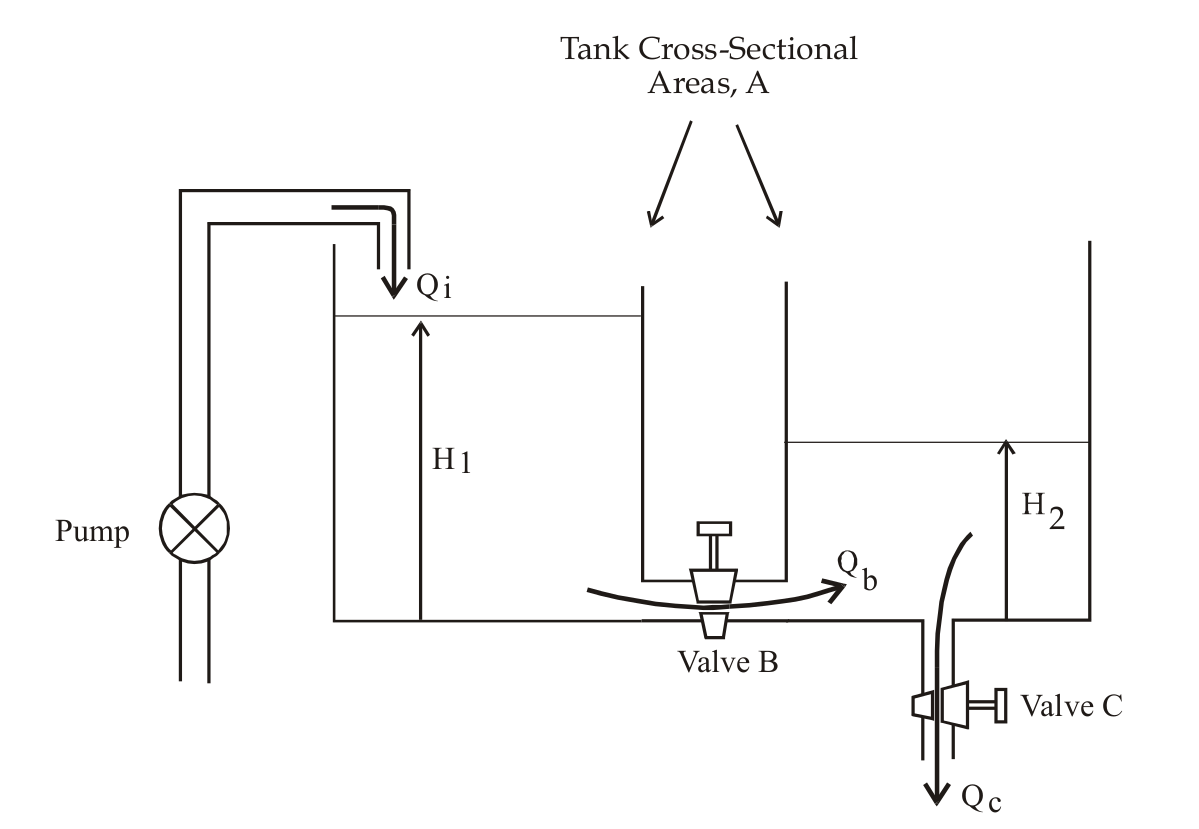
\includegraphics[scale=.3]{baitap3-2binhchua}
        \end{center}
        \caption{Hệ thống 2 bình chứa} \label{baitap3-2binhchua}
    \end{figure}

\paragraph{Yêu cầu}
    \begin{enumerate}[a.]
        \item Xác định các biến vào, biến ra, biến điều khiển, biến cần điều khiển và biến nhiễu.
        \item Viết phương trình động học cho mức chất lỏng trong bồn chứa.
        \item Tuyến tính hóa phương trình xây dựng được xung quanh vị trí cân bằng dựa trên phương pháp khai triển Taylor.
        \item Xác định hàm truyền $G(s) = \dfrac{H_2(s)}{Q_i(s)}$
    \end{enumerate}

\paragraph{Bài giải}
    \begin{enumerate}[\it a.]
        \item \textit{Xác định các biến vào, biến ra, biến điều khiển, biến cần điều khiển và biến nhiễu.}
            \begin{itemize}
                \item Biến vào: $Q_i, Q_b, Q_c$.
                \item Biến ra: $H_1, H_2$.
                \item Biến điều khiển: $Q_b, Q_c$.
                \item Biến cần điều khiển: $H_1, H_2$.
                \item Biến nhiễu: $Q_i$.
            \end{itemize}

        \item \textit{Viết phương trình động học cho mức chất lỏng trong bồn chứa.}
            \begin{itemize}
                \item Phương trình cho bình chứa 1:
                    \begin{itemize}
                        \item Bình chứa 1:
                            \begin{align} \label{eq:baitap3-2binhchua}
                                \frac{dV_1}{dt} = Q_i - Q_b \Longleftrightarrow \dfrac{d\left({A_1 H_1}\right)}{dt} = Q_i - Q_b \Longleftrightarrow \dfrac{dH_1}{dt} = \dfrac{1}{A_1} \left({Q_i - Q_b}\right)
                            \end{align}

                        \item Thay $Q_b = C_{db}a_b\sqrt{2g(H_1 - H_2)}$ vào (\ref{eq:baitap3-2binhchua}), ta có:
                            \begin{align}
                                \dfrac{dH_1}{dt} = \dfrac{1}{A_1} \left({Q_i - Q_b}\right) = \dfrac{1}{A_1} \left[{Q_i - C_{db}a_b\sqrt{2g(H_1 - H_2)}}\right]
                            \end{align}
                    \end{itemize}

                \item Phương trình cho bình chứa 2:
                    \begin{itemize}
                        \item Bình chứa 2:
                            \begin{align} \label{eq:baitap3-2binhchua-2}
                                \dfrac{dV_2}{dt} = Q_b - Q_c \Longleftrightarrow \dfrac{d\left({A_2 H_2}\right)}{dt} = Q_b - Q_c \Longleftrightarrow \dfrac{dH_2}{dt} = \dfrac{1}{A_2} \left({Q_b - Q_c}\right)
                            \end{align}

                        \item Thay $Q_b = C_{db}a_b\sqrt{2g(H_1 - H_2)}$ và $Q_c = C_{dc}a_c\sqrt{2gH_2}$ vào (\ref{eq:baitap3-2binhchua-2}), ta có:
                            \begin{align}
                                \dfrac{dH_2}{dt} = \dfrac{1}{A_2} \left({Q_b - Q_c}\right) = \dfrac{1}{A_2} \left[{C_{db}a_b\sqrt{2g(H_1 - H_2)} - C_{dc}a_c\sqrt{2gH_2}}\right]
                            \end{align}
                    \end{itemize}

                \item Kết luận, hệ phương trình mô tả quá trình:
                    \begin{align}
                        \left\{
                        \begin{array}{l}
                            \dfrac{dH_1}{dt} = \dfrac{1}{A_1} \left[{Q_i - C_{db}a_b\sqrt{2g(H_1 - H_2)}}\right]\\ [.5cm]
                            \dfrac{dH_2}{dt} = \dfrac{1}{A_2} \left[{C_{db}a_b\sqrt{2g(H_1 - H_2)} - C_{dc}a_c\sqrt{2gH_2}}\right]
                        \end{array}
                        \right.
                    \end{align}
            \end{itemize}

        \item \textit{Tuyến tính hóa phương trình xây dựng được xung quanh vị trí cân bằng dựa trên phương pháp khai triển Taylor.}
            \begin{itemize}
                \item Gọi $\left({\overline{Q_i}, \overline{H_1}, \overline{H_2}}\right)$ là điểm làm việc cân bằng của hệ thống gồm 2 bình chứa.

                \item Gọi $Q_i = \overline{Q_i} + \Delta Q_i, H_1 = \overline{H_1} + \Delta H_1, H_2 = \overline{H_2} + \Delta H_2$.

                \item Đặt $f\left({Q_i, H_1, H_2}\right) = \dot{H_1} = \dfrac{1}{A_1} \left[{Q_i - C_{db}a_b\sqrt{2g(H_1 - H_2)}}\right]$
                    \begin{itemize}
                        \item Tại điểm làm việc cân bằng $\left({\overline{Q_i}, \overline{H_1}, \overline{H_2}}\right)$ thì
                            \begin{align}
                                f\left({\overline{Q_i}, \overline{H_1}, \overline{H_2}}\right) = 0 \Longleftrightarrow \dfrac{1}{A_1} \left[{\overline{Q_i} - C_{db}a_b\sqrt{2g(\overline{H_1} - \overline{H_2})}}\right] = 0
                            \end{align}

                        \item Khai triển Taylor cho $f\left({Q_i, H_1, H_2}\right) = \dot{H_1} = \dfrac{1}{A_1} \left[{Q_i - C_{db}a_b\sqrt{2g(H_1 - H_2)}}\right]$, ta có:
                            \begin{align}
                                \dot{H_1} = \Delta \dot{H_1} & = f\left({\overline{Q_i} + \Delta Q_i, \overline{H_1} + \Delta H_1, \overline{H_2} + \Delta H_2}\right) \\
                                & \approx \underbrace{f\left({\overline{Q_i}, \overline{H_1}, \overline{H_2}}\right)}_{0} + \left.\dfrac{\partial f}{\partial Q_i}\right|_{\left({\overline{Q_i}, \overline{H_1}, \overline{H_2}}\right)} \Delta Q_i + \left.\dfrac{\partial f}{\partial H_1}\right|_{\left({\overline{Q_i}, \overline{H_1}, \overline{H_2}}\right)} \Delta H_1 + \left.\dfrac{\partial f}{\partial H_2}\right|_{\left({\overline{Q_i}, \overline{H_1}, \overline{H_2}}\right)} \Delta H_2\\
                                & \approx \dfrac{1}{A_1} \left[{\Delta Q_i - \dfrac{2gC_{db}a_b}{2\sqrt{2g(\overline{H_1} - \overline{H_2})}} \Delta H_1 + \dfrac{2gC_{db}a_b}{2\sqrt{2g(\overline{H_1} - \overline{H_2})}} \Delta H_2}\right]\\
                                & \approx \dfrac{1}{A_1} \left[{\Delta Q_i - \dfrac{gC_{db}a_b}{\sqrt{2g(\overline{H_1} - \overline{H_2})}} \Delta H_1 + \dfrac{gC_{db}a_b}{\sqrt{2g(\overline{H_1} - \overline{H_2})}} \Delta H_2}\right]
                            \end{align}

                        \item Kết luận:
                            \begin{align}
                                \Delta \dot{H_1} = \dfrac{1}{A_1} \left[{\Delta Q_i - \dfrac{gC_{db}a_b}{\sqrt{2g(\overline{H_1} - \overline{H_2})}} \Delta H_1 + \dfrac{gC_{db}a_b}{\sqrt{2g(\overline{H_1} - \overline{H_2})}} \Delta H_2}\right]
                            \end{align}
                    \end{itemize}

                \item Đặt $g\left({Q_i, H_1, H_2}\right) = \dot{H_2} = \dfrac{1}{A_2} \left[{C_{db}a_b\sqrt{2g(H_1 - H_2)} - C_{dc}a_c\sqrt{2gH_2}}\right]$
                    \begin{itemize}
                        \item Tại điểm làm việc cân bằng $\left({\overline{Q_i}, \overline{H_1}, \overline{H_2}}\right)$ thì:
                            \begin{align}
                                g\left({\overline{Q_i}, \overline{H_1}, \overline{H_2}}\right) = 0 \Longleftrightarrow \dfrac{1}{A_2} \left[{C_{db}a_b\sqrt{2g(\overline{H_1} - \overline{H_2})} - C_{dc}a_c\sqrt{2g \overline{H_2}}}\right] = 0
                            \end{align}

                        \item Khai triển Taylor cho $g\left({Q_i, H_1, H_2}\right) = \dot{H_2} = \dfrac{1}{A_2} \left[{C_{db}a_b\sqrt{2g(H_1 - H_2)} - C_{dc}a_c\sqrt{2gH_2}}\right]$, ta có:
                            \begin{align}
                                \dot{H_2} = \Delta \dot{H_2} & = g\left({\overline{Q_i} + \Delta Q_i, \overline{H_1} + \Delta H_1, \overline{H_2} + \Delta H_2}\right) \\
                                & \approx \underbrace{g\left({\overline{Q_i}, \overline{H_1}, \overline{H_2}}\right)}_{0} + \left.\dfrac{\partial g}{\partial H_1}\right|_{\left({\overline{Q_i}, \overline{H_1}, \overline{H_2}}\right)} \Delta H_1 + \left.\dfrac{\partial g}{\partial H_2}\right|_{\left({\overline{Q_i}, \overline{H_1}, \overline{H_2}}\right)} \Delta H_2\\
                                & \approx \dfrac{1}{A_2} \left[{\dfrac{2g C_{db}a_b}{2 \sqrt{2g(\overline{H_1} - \overline{H_2})}} \Delta H_1 + \dfrac{-2g C_{db}a_b}{2 \sqrt{2g(\overline{H_1} - \overline{H_2})}} \Delta H_2 - \dfrac{2g C_{dc}a_c}{2 \sqrt{2g\overline{H_2}}} \Delta H_2}\right]\\
                                & \approx \dfrac{1}{A_2} \left[{\dfrac{g C_{db}a_b}{\sqrt{2g(\overline{H_1} - \overline{H_2})}} \Delta H_1 - \dfrac{g C_{db}a_b}{\sqrt{2g(\overline{H_1} - \overline{H_2})}} \Delta H_2 - \dfrac{g C_{dc}a_c}{\sqrt{2g\overline{H_2}}} \Delta H_2}\right]
                            \end{align}

                        \item Kết luận:
                            \begin{align}
                                \Delta \dot{H_2} = \dfrac{1}{A_2} \left[{\dfrac{g C_{db}a_b}{\sqrt{2g(\overline{H_1} - \overline{H_2})}} \Delta H_1 - \dfrac{g C_{db}a_b}{\sqrt{2g(\overline{H_1} - \overline{H_2})}} \Delta H_2 - \dfrac{g C_{dc}a_c}{\sqrt{2g\overline{H_2}}} \Delta H_2}\right]
                            \end{align}
                    \end{itemize}

                \item Kết luận, phương trình tuyến tính hóa của mô hình tại điểm làm việc cân bằng $\left({\overline{Q_i}, \overline{H_1}, \overline{H_2}}\right)$:
                    \begin{align}
                        \left\{
                        \begin{array}{l}
                            \Delta \dot{H_1} = \dfrac{1}{A_1} \left[{\Delta Q_i - \dfrac{gC_{db}a_b}{\sqrt{2g(\overline{H_1} - \overline{H_2})}} \Delta H_1 + \dfrac{gC_{db}a_b}{\sqrt{2g(\overline{H_1} - \overline{H_2})}} \Delta H_2}\right]\\ [.5cm]
                            \Delta \dot{H_2} = \dfrac{1}{A_2} \left[{\dfrac{g C_{db}a_b}{\sqrt{2g(\overline{H_1} - \overline{H_2})}} \Delta H_1 - \dfrac{g C_{db}a_b}{\sqrt{2g(\overline{H_1} - \overline{H_2})}} \Delta H_2 - \dfrac{g C_{dc}a_c}{\sqrt{2g\overline{H_2}}} \Delta H_2}\right]
                        \end{array}
                        \right.
                    \end{align}
            \end{itemize}

        \item \textit{Xác định hàm truyền $G(s) = \dfrac{H_2(s)}{Q_i(s)}$}
            \begin{itemize}
                \item Ta có: $\Delta \dot{H_1} = \dfrac{1}{A_1} \left[{\Delta Q_i - \dfrac{gC_{db}a_b}{\sqrt{2g(\overline{H_1} - \overline{H_2})}} \Delta H_1 + \dfrac{gC_{db}a_b}{\sqrt{2g(\overline{H_1} - \overline{H_2})}} \Delta H_2}\right]$, thực hiện biến đổi Laplace 2 vế của phương trình ta có:
                    \begin{align}
                        & s H_1(s) = \dfrac{1}{A_1} \left[{Q_i(s) - \dfrac{gC_{db}a_b}{\sqrt{2g(\overline{H_1} - \overline{H_2})}} H_1(s) + \dfrac{gC_{db}a_b}{\sqrt{2g(\overline{H_1} - \overline{H_2})}} H_2(s)}\right]\\
                        \Longleftrightarrow & s A_1 H_1(s) + \dfrac{gC_{db}a_b}{\sqrt{2g(\overline{H_1} - \overline{H_2})}} H_1(s) = Q_i(s) + \dfrac{gC_{db}a_b}{\sqrt{2g(\overline{H_1} - \overline{H_2})}} H_2(s)\\
                        \Longleftrightarrow & \left[{s A_1 + \dfrac{gC_{db}a_b}{\sqrt{2g(\overline{H_1} - \overline{H_2})}}}\right] H_1(s) = Q_i(s) + \dfrac{gC_{db}a_b}{\sqrt{2g(\overline{H_1} - \overline{H_2})}} H_2(s) \\
                        \Longleftrightarrow & H_1(s) = \dfrac{Q_i(s) + \dfrac{gC_{db}a_b}{\sqrt{2g(\overline{H_1} - \overline{H_2})}} H_2(s)}{s A_1 + \dfrac{gC_{db}a_b}{\sqrt{2g(\overline{H_1} - \overline{H_2})}}}
                    \end{align}

                \item Ta có: $\Delta \dot{H_2} = \dfrac{1}{A_2} \left[{\dfrac{g C_{db}a_b}{\sqrt{2g(\overline{H_1} - \overline{H_2})}} \Delta H_1 - \dfrac{g C_{db}a_b}{\sqrt{2g(\overline{H_1} - \overline{H_2})}} \Delta H_2 - \dfrac{g C_{dc}a_c}{\sqrt{2g\overline{H_2}}} \Delta H_2}\right]$, thực hiện biến đổi Laplace 2 vế của phương trình ta có:
                    \begin{align}
                        & s H_2(s) = \dfrac{1}{A_2} \left[{\dfrac{g C_{db}a_b}{\sqrt{2g(\overline{H_1} - \overline{H_2})}} H_1(s) - \dfrac{g C_{db}a_b}{\sqrt{2g(\overline{H_1} - \overline{H_2})}} H_2(s) - \dfrac{g C_{dc}a_c}{\sqrt{2g\overline{H_2}}} H_2(s)}\right] \\
                        \Longleftrightarrow & s A_2 H_2(s) + \dfrac{g C_{db}a_b}{\sqrt{2g(\overline{H_1} - \overline{H_2})}} H_2(s) + \dfrac{g C_{dc}a_c}{\sqrt{2g\overline{H_2}}} H_2(s) = \dfrac{g C_{db}a_b}{\sqrt{2g(\overline{H_1} - \overline{H_2})}} H_1(s) \\
                        \Longleftrightarrow & \left[{s A_2 + \dfrac{g C_{db}a_b}{\sqrt{2g(\overline{H_1} - \overline{H_2})}} + \dfrac{g C_{dc}a_c}{\sqrt{2g\overline{H_2}}}}\right] H_2(s) = \dfrac{g C_{db}a_b}{\sqrt{2g(\overline{H_1} - \overline{H_2})}} H_1(s) \\
                        \Longleftrightarrow & \dfrac{\sqrt{2g(\overline{H_1} - \overline{H_2})}}{g C_{db}a_b} \left[{s A_2 + \dfrac{g C_{db}a_b}{\sqrt{2g(\overline{H_1} - \overline{H_2})}} + \dfrac{g C_{dc}a_c}{\sqrt{2g\overline{H_2}}}}\right] H_2(s) = H_1(s) \\
                        \Longleftrightarrow & \dfrac{\sqrt{2g(\overline{H_1} - \overline{H_2})}}{g C_{db}a_b} \left[{s A_2 + \dfrac{g C_{db}a_b}{\sqrt{2g(\overline{H_1} - \overline{H_2})}} + \dfrac{g C_{dc}a_c}{\sqrt{2g\overline{H_2}}}}\right] H_2(s) = \dfrac{Q_i(s) + \dfrac{gC_{db}a_b}{\sqrt{2g(\overline{H_1} - \overline{H_2})}} H_2(s)}{s A_1 + \dfrac{gC_{db}a_b}{\sqrt{2g(\overline{H_1} - \overline{H_2})}}} \\
                        \Longleftrightarrow & \dfrac{\sqrt{2g(\overline{H_1} - \overline{H_2})}}{g C_{db}a_b} \left[{s A_1 + \dfrac{gC_{db}a_b}{\sqrt{2g(\overline{H_1} - \overline{H_2})}}}\right] \left[{s A_2 + \dfrac{g C_{db}a_b}{\sqrt{2g(\overline{H_1} - \overline{H_2})}} + \dfrac{g C_{dc}a_c}{\sqrt{2g\overline{H_2}}}}\right] H_2(s) \nonumber \\
                        & = Q_i(s) + \dfrac{gC_{db}a_b}{\sqrt{2g(\overline{H_1} - \overline{H_2})}} H_2(s) \\
                        \Longleftrightarrow & \dfrac{\sqrt{2g(\overline{H_1} - \overline{H_2})}}{g C_{db}a_b} \left[{s A_1 + \dfrac{gC_{db}a_b}{\sqrt{2g(\overline{H_1} - \overline{H_2})}}}\right] \left[{s A_2 + \dfrac{g C_{db}a_b}{\sqrt{2g(\overline{H_1} - \overline{H_2})}} + \dfrac{g C_{dc}a_c}{\sqrt{2g\overline{H_2}}}}\right] H_2(s) \nonumber \\
                        & - \dfrac{gC_{db}a_b}{\sqrt{2g(\overline{H_1} - \overline{H_2})}} H_2(s) = Q_i(s) \\
                        \Longleftrightarrow & \left\{{\dfrac{\sqrt{2g(\overline{H_1} - \overline{H_2})}}{g C_{db}a_b} \left[{s A_1 + \dfrac{gC_{db}a_b}{\sqrt{2g(\overline{H_1} - \overline{H_2})}}}\right] \left[{s A_2 + \dfrac{g C_{db}a_b}{\sqrt{2g(\overline{H_1} - \overline{H_2})}} + \dfrac{g C_{dc}a_c}{\sqrt{2g\overline{H_2}}}}\right]}\right. \nonumber \\
                        & \left.{- \dfrac{gC_{db}a_b}{\sqrt{2g(\overline{H_1} - \overline{H_2})}}}\right\} H_2(s) = Q_i(s) \\
                        \Longleftrightarrow & \dfrac{H_2(s)}{Q_i(s)} = \nonumber \\
                        & \dfrac{1}{\dfrac{\sqrt{2g(\overline{H_1} - \overline{H_2})}}{g C_{db}a_b} \left[{s A_1 + \dfrac{gC_{db}a_b}{\sqrt{2g(\overline{H_1} - \overline{H_2})}}}\right] \left[{s A_2 + \dfrac{g C_{db}a_b}{\sqrt{2g(\overline{H_1} - \overline{H_2})}} + \dfrac{g C_{dc}a_c}{\sqrt{2g\overline{H_2}}}}\right] - \dfrac{gC_{db}a_b}{\sqrt{2g(\overline{H_1} - \overline{H_2})}}}
                    \end{align}

                \item Kết luận:
                    \begin{align}
                        G(s) & = \dfrac{H_2(s)}{Q_i(s)} \nonumber\\
                        & = \dfrac{1}{\dfrac{\sqrt{2g(\overline{H_1} - \overline{H_2})}}{g C_{db}a_b} \left[{s A_1 + \dfrac{gC_{db}a_b}{\sqrt{2g(\overline{H_1} - \overline{H_2})}}}\right] \left[{s A_2 + \dfrac{g C_{db}a_b}{\sqrt{2g(\overline{H_1} - \overline{H_2})}} + \dfrac{g C_{dc}a_c}{\sqrt{2g\overline{H_2}}}}\right] - \dfrac{gC_{db}a_b}{\sqrt{2g(\overline{H_1} - \overline{H_2})}}}
                    \end{align}
            \end{itemize}
    \end{enumerate}


\section{Bài tập \ref{sec:baitap4-2binhchua}} \label{sec:baitap4-2binhchua}
    \paragraph{Giả thiết}
    Cho hệ thống như hình \ref{Fig:baitap4-2binhchua}: Các lưu lượng ra $q_1$ và $q_0$ được xác định như sau: $q_1 = \dfrac{h_1 - h_2}{R_1}$ và $q_0 = \dfrac{h_2}{R_2}$
    \begin{figure}[htp]
        \begin{center}
            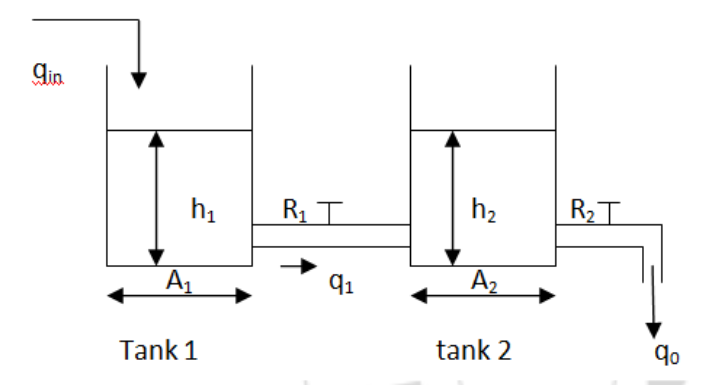
\includegraphics[scale=.5]{baitap4-2binhchua}
        \end{center}
        \caption{Hệ thống 2 bình chứa} \label{Fig:baitap4-2binhchua}
    \end{figure}

\paragraph{Yêu cầu}
    \begin{enumerate}[a.]
        \item Xác định các biến vào, biến ra, biến điều khiển, biến cần điều khiển và biến nhiễu.
        \item Viết phương trình động học cho mức chất lỏng trong bồn chứa.
        \item Nếu phương trình phi tuyến hãy tuyến tính hóa phương trình xây dựng được xung quanh vị trí cân bằng dựa trên phương pháp khai triển Taylor.
        \item Xác định hàm truyền $G(s) = \dfrac{H_2(s)}{Q_{in}(s)}$
    \end{enumerate}

\paragraph{Bài giải}
    \begin{enumerate}[\it a.]
        \item \textit{Xác định các biến vào, biến ra, biến điều khiển, biến cần điều khiển và biến nhiễu.}
            \begin{itemize}
                \item Biến vào: $q_{in}, q_1, q_0$.
                \item Biến ra: $h_1, h_2$.
                \item Biến điều khiển: $q_1, q_0$.
                \item Biến cần điều khiển: $h_1, h_2$.
                \item Biến nhiễu: $q_{in}$.
            \end{itemize}

        \item \textit{Viết phương trình động học cho mức chất lỏng trong bồn chứa.}
            \begin{itemize}
                \item Phương trình cho bình chứa 1:
                    \begin{itemize}
                        \item Bình chứa 1:
                            \begin{align} \label{eq:baitap4-2binhchua-1}
                                \frac{dV_1}{dt} = q_{in} - q_1 \Longleftrightarrow \dfrac{d\left({A_1 h_1}\right)}{dt} = q_{in} - q_1 \Longleftrightarrow \dfrac{dh_1}{dt} = \dfrac{1}{A_1} \left({q_{in} - q_1}\right)
                            \end{align}

                        \item Thay $q_1 = \dfrac{h_1 - h_2}{R_1}$ vào (\ref{eq:baitap4-2binhchua-1}), ta có:
                            \begin{align} \label{eq:baitap4-2binhchua-2}
                                \dfrac{dh_1}{dt} = \dfrac{1}{A_1} \left({q_{in} - q_1}\right) = \dfrac{1}{A_1} \left({q_{in} - \dfrac{h_1 - h_2}{R_1}}\right)
                            \end{align}
                    \end{itemize}

                \item Phương trình cho bình chứa 2:
                    \begin{itemize}
                        \item Bình chứa 2:
                            \begin{align} \label{eq:baitap4-2binhchua-3}
                                \dfrac{dV_2}{dt} = q_1 - q_0 \Longleftrightarrow \dfrac{d\left({A_2 h_2}\right)}{dt} = q_1 - q_0 \Longleftrightarrow \dfrac{dh_2}{dt} = \dfrac{1}{A_2} \left({q_1 - q_0}\right)
                            \end{align}

                        \item Thay $q_1 = \dfrac{h_1 - h_2}{R_1}$ và $q_0 = \dfrac{h_2}{R_2}$ vào (\ref{eq:baitap4-2binhchua-3}), ta có:
                            \begin{align}
                                \dfrac{dh_2}{dt} = \dfrac{1}{A_2} \left({q_1 - q_0}\right) = \dfrac{1}{A_2} \left({\dfrac{h_1 - h_2}{R_1} - \dfrac{h_2}{R_2}}\right)
                            \end{align}
                    \end{itemize}

                \item Kết luận, hệ phương trình mô tả quá trình:
                    \begin{align}
                        \left\{
                        \begin{array}{l}
                            \dfrac{dh_1}{dt} = \dfrac{1}{A_1} \left({q_{in} - \dfrac{h_1 - h_2}{R_1}}\right)\\ [.5cm]
                            \dfrac{dh_2}{dt} = \dfrac{1}{A_2} \left({\dfrac{h_1 - h_2}{R_1} - \dfrac{h_2}{R_2}}\right)
                        \end{array}
                        \right.
                    \end{align}
            \end{itemize}

        \item \textit{Nếu phương trình phi tuyến hãy tuyến tính hóa phương trình xây dựng được xung quanh vị trí cân bằng dựa trên phương pháp khai triển Taylor.}
            \begin{itemize}
                \item Ta có:
                    \begin{align}\label{eq:baitap4-2binhchua-4}
                        \left\{
                        \begin{array}{l}
                            \dfrac{dh_1}{dt} = \dfrac{1}{A_1} \left({q_{in} - \dfrac{h_1 - h_2}{R_1}}\right)\\ [.5cm]
                            \dfrac{dh_2}{dt} = \dfrac{1}{A_2} \left({\dfrac{h_1 - h_2}{R_1} - \dfrac{h_2}{R_2}}\right)
                        \end{array}
                        \right.
                        \Longleftrightarrow
                        \left\{
                        \begin{array}{l}
                            \dfrac{dh_1}{dt} = \dfrac{1}{A_1} \left({q_{in} - \dfrac{1}{R_1} h_1 + \dfrac{1}{R_1} h_2}\right)\\ [.5cm]
                            \dfrac{dh_2}{dt} = \dfrac{1}{A_2} \left[{\dfrac{1}{R_1} h_1 - \left({\dfrac{1}{R_1} + \dfrac{1}{R_2}}\right) h_2}\right]
                        \end{array}
                        \right.
                    \end{align}

                \item Do hệ phương trình (\ref{eq:baitap4-2binhchua-4}) đã tuyến tính rồi nên ta không cần phải tuyến tính hóa.

                \item Nếu ta đi tuyến tính hóa hệ phương trình (\ref{eq:baitap4-2binhchua-4}) thì cho kết quả không thay đổi.
                    \begin{itemize}
                        \item Gọi $\left({\overline{q_{in}}, \overline{h_1}, \overline{h_2}}\right)$ là điểm làm việc cân bằng của hệ thống gồm 2 bình chứa.

                        \item Gọi $q_{in} = \overline{q_{in}} + \Delta q_{in}, h_1 = \overline{h_1} + \Delta h_1, h_2 = \overline{h_2} + \Delta h_2$.

                        \item Đặt $f\left({q_{in}, h_1, h_2}\right) = \dot{h_1} = \dfrac{1}{A_1} \left({q_{in} - \dfrac{h_1 - h_2}{R_1}}\right)$
                            \begin{itemize}
                                \item Tại điểm làm việc cân bằng $\left({\overline{q_{in}}, \overline{h_1}, \overline{h_2}}\right)$ thì
                                    \begin{align}
                                        f\left({\overline{q_{in}}, \overline{h_1}, \overline{h_2}}\right) = 0 \Longleftrightarrow \dfrac{1}{A_1} \left({\overline{q_{in}} - \dfrac{\overline{h_1} - \overline{h_2}}{R_1}}\right) = 0
                                    \end{align}

                                \item Khai triển Taylor cho $f\left({q_{in}, h_1, h_2}\right) = \dot{h_1} = \dfrac{1}{A_1} \left({q_{in} - \dfrac{h_1 - h_2}{R_1}}\right)$, ta có:
                                    \begin{align}
                                        \dot{h_1} = \Delta h_1 & = f\left({\overline{q_{in}} + \Delta q_{in}, \overline{h_1} + \Delta h_1, \overline{h_2} + \Delta h_2}\right) \\
                                        & \approx \underbrace{f\left({\overline{q_{in}}, \overline{h_1}, \overline{h_2}}\right)}_{0} + \left.\dfrac{\partial f}{\partial q_{in}}\right|_{\left({\overline{q_{in}}, \overline{h_1}, \overline{h_2}}\right)} \Delta q_{in} + \left.\dfrac{\partial f}{\partial h_1}\right|_{\left({\overline{q_{in}}, \overline{h_1}, \overline{h_2}}\right)} \Delta h_1 + \left.\dfrac{\partial f}{\partial h_2}\right|_{\left({\overline{q_{in}}, \overline{h_1}, \overline{h_2}}\right)} \Delta h_2\\
                                        & \approx \dfrac{1}{A_1} \left({\Delta q_{in} - \dfrac{\Delta h_1}{R_1} + \dfrac{\Delta h_2}{R_1}}\right)\\
                                    \end{align}

                                \item Thay $\Delta q_{in} = q_{in}, \Delta h_1 = h_1$ và $\Delta h_2 = h_2$, ta có:
                                    \begin{align}
                                        \dfrac{dh_1}{dt} = \dfrac{1}{A_1} \left({q_{in} - \dfrac{h_1}{R_1} + \dfrac{h_2}{R_1}}\right)
                                    \end{align}
                            \end{itemize}

                        \item Đặt $g\left({q_{in}, h_1, h_2}\right) = \dot{h_2} = \dfrac{1}{A_2} \left({\dfrac{h_1 - h_2}{R_1} - \dfrac{h_2}{R_2}}\right)$
                            \begin{itemize}
                                \item Tại điểm làm việc cân bằng $\left({\overline{q_{in}}, \overline{h_1}, \overline{h_2}}\right)$ thì:
                                    \begin{align}
                                        g\left({\overline{q_{in}}, \overline{h_1}, \overline{h_2}}\right) = 0 \Longleftrightarrow \dfrac{1}{A_2} \left({\dfrac{\overline{h_1} - \overline{h_2}}{R_1} - \dfrac{\overline{h_2}}{R_2}}\right) = 0
                                    \end{align}

                                \item Khai triển Taylor cho $g\left({q_{in}, h_1, h_2}\right) = \dot{h_2} = \dfrac{1}{A_2} \left({\dfrac{h_1 - h_2}{R_1} - \dfrac{h_2}{R_2}}\right)$, ta có:
                                    \begin{align}
                                        \dot{h_2} = \Delta h_2 & = g\left({\overline{q_{in}} + \Delta q_{in}, \overline{h_1} + \Delta h_1, \overline{h_2} + \Delta h_2}\right) \\
                                        & \approx \underbrace{g\left({\overline{q_{in}}, \overline{h_1}, \overline{h_2}}\right)}_{0} + \left.\dfrac{\partial g}{\partial h_1}\right|_{\left({\overline{q_{in}}, \overline{h_1}, \overline{h_2}}\right)} \Delta h_1 + \left.\dfrac{\partial g}{\partial h_2}\right|_{\left({\overline{q_{in}}, \overline{h_1}, \overline{h_2}}\right)} \Delta h_2\\
                                        & \approx \dfrac{1}{A_2} \left({\dfrac{\Delta h_1}{R_1} - \dfrac{\Delta h_2}{R_1} - \dfrac{\Delta h_2}{R_2}}\right)\\
                                        & \approx \dfrac{1}{A_2} \left[{\dfrac{\Delta h_1}{R_1} - \left({\dfrac{1}{R_1} + \dfrac{1}{R_2}}\right) \Delta h_2}\right]
                                    \end{align}

                                \item Thay $\Delta h_1= h_1$ và $\Delta h_2 = h_2$, ta có:
                                    \begin{align}
                                        \dfrac{dh_2}{dt} = \dfrac{1}{A_2} \left[{\dfrac{h_1}{R_1} - \left({\dfrac{1}{R_1} + \dfrac{1}{R_2}}\right) h_2}\right]
                                    \end{align}
                            \end{itemize}

                        \item Kết luận, phương trình tuyến tính hóa của mô hình tại điểm làm việc cân bằng $\left({\overline{q_{in}}, \overline{h_1}, \overline{h_2}}\right)$:
                            \begin{align}
                                \left\{
                                \begin{array}{l}
                                    \dfrac{dh_1}{dt} = \dfrac{1}{A_1} \left({q_{in} - \dfrac{h_1}{R_1} + \dfrac{h_2}{R_1}}\right)\\ [.5cm]
                                    \dfrac{dh_2}{dt} = \dfrac{1}{A_2} \left[{\dfrac{h_1}{R_1} - \left({\dfrac{1}{R_1} + \dfrac{1}{R_2}}\right) h_2}\right]
                                \end{array}
                                \right.
                            \end{align}
                \end{itemize}
            \end{itemize}

        \item \textit{Xác định hàm truyền $G(s) = \dfrac{h_2(s)}{Q_{in}(s)}$}
            \begin{itemize}
                \item Ta có: $\dfrac{dh_1}{dt} = \dfrac{1}{A_1} \left({q_{in} - \dfrac{h_1}{R_1}}\right)$, thực hiện biến đổi Laplace 2 vế của phương trình ta có:
                    \begin{align}
                        & s H_1(s) = \dfrac{1}{A_1} \left[{Q_{in}(s) - \dfrac{H_1(s)}{R_1} + \dfrac{H_2(s)}{R_1}}\right]\\
                        \Longleftrightarrow & s A_1 H_1(s) + \dfrac{1}{R_1} H_1(s) = Q_{in}(s) + \dfrac{H_2(s)}{R_1}\\
                        \Longleftrightarrow & \left({s A_1 + \dfrac{1}{R_1}}\right) H_1(s) = Q_{in}(s) + \dfrac{H_2(s)}{R_1} \\
                        \Longleftrightarrow & H_1(s) = \frac{Q_{in}(s) + \dfrac{H_2(s)}{R_1} }{s A_1 + \dfrac{1}{R_1}}
                    \end{align}

                \item Ta có: $\dfrac{dh_2}{dt} = \dfrac{1}{A_2} \left[{\dfrac{h_1}{R_1} - \left({\dfrac{1}{R_1} + \dfrac{1}{R_2}}\right) h_2}\right]$, thực hiện biến đổi Laplace 2 vế của phương trình ta có:
                    \begin{align}
                        & s H_2(s) = \dfrac{1}{A_2} \left[{\dfrac{H_1(s)}{R_1} - \left({\dfrac{1}{R_1} + \dfrac{1}{R_2}}\right) H_2(s)}\right] \\
                        \Longleftrightarrow & s A_2 H_2(s) + \left({\dfrac{1}{R_1} + \dfrac{1}{R_2}}\right) H_2(s) = \dfrac{H_1(s)}{R_1} \\
                        \Longleftrightarrow & \left[{s A_2 + \left({\dfrac{1}{R_1} + \dfrac{1}{R_2}}\right)}\right] H_2(s) = \dfrac{H_1(s)}{R_1}\\
                        \Longleftrightarrow & \left[{s A_2 + \left({\dfrac{1}{R_1} + \dfrac{1}{R_2}}\right)}\right] H_2(s) = \frac{Q_{in}(s) + \dfrac{H_2(s)}{R_1}}{R_1 \left({s A_1 + \dfrac{1}{R_1}}\right)}\\
                        \Longleftrightarrow & \left[{s A_2 + \left({\dfrac{1}{R_1} + \dfrac{1}{R_2}}\right)}\right] H_2(s) = \frac{Q_{in}(s) + \dfrac{H_2(s)}{R_1}}{s A_1 R_1 + 1}\\
                        \Longleftrightarrow & \left({s A_1 R_1 + 1}\right) \left[{s A_2 + \left({\dfrac{1}{R_1} + \dfrac{1}{R_2}}\right)}\right] H_2(s) = Q_{in}(s) + \dfrac{H_2(s)}{R_1}\\
                        \Longleftrightarrow & \left({s A_1 R_1 + 1}\right) \left[{s A_2 + \left({\dfrac{1}{R_1} + \dfrac{1}{R_2}}\right)}\right] H_2(s) - \dfrac{H_2(s)}{R_1} = Q_{in}(s)\\
                        \Longleftrightarrow & \left\{{\left({s A_1 R_1 + 1}\right) \left[{s A_2 + \left({\dfrac{1}{R_1} + \dfrac{1}{R_2}}\right)}\right] - \dfrac{1}{R_1}}\right\}H_2(s) = Q_{in}(s)\\
                        \Longleftrightarrow & \dfrac{H_2(s)}{Q_{in}(s)} = \dfrac{1}{\left({s A_1 R_1 + 1}\right) \left[{s A_2 + \left({\dfrac{1}{R_1} + \dfrac{1}{R_2}}\right)}\right] - \dfrac{1}{R_1}}
                    \end{align}

                \item Kết luận:
                    \begin{align}
                        G(s) = \dfrac{H_2(s)}{Q_{in}(s)} = \dfrac{1}{\left({s A_1 R_1 + 1}\right) \left[{s A_2 + \left({\dfrac{1}{R_1} + \dfrac{1}{R_2}}\right)}\right] - \dfrac{1}{R_1}}
                    \end{align}
            \end{itemize}
    \end{enumerate}


\end{document}
